\input{bctcs08-slides.pre}
\def\toolname{HOG}

\pstrSetArrowColor{black}

\title{\texorpdfstring{A Concrete Presentation of Game Semantics}{A Concrete Presentation of Game Semantics}}

\author[W. Blum, C.-H. L. Ong]{\texorpdfstring{\\ William Blum\\ \ \\
 Joint work with C.-H. Luke Ong}{William Blum}}


\institute[Oxford University -- Edinburgh University]{School of Informatics, University of Edinburgh -- Oxford University Computing Laboratory}

\date{\small \color{red}{BCTCS, 8 April 2008}}


\begin{document}

\frame{\titlepage}

\frame{\frametitle{Overview}
\begin{itemize}
  \item
Game-semantic models are \highlight{abstract} \ie independent of the syntax of the denotated term. We give here a \highlight{concrete} \ie syntactic representation of game semantics where:
\begin{itemize}
\item The arena game is `incarnated' by some abstract syntax tree of the term,
\item Uncovered plays are given by traversals over this tree.
\end{itemize}


\item A ``Correspondence Theorem'' establishes the relationship between the game-semantic and traversal models.

\item The tool \toolname\ illustrates this correspondence.
\end{itemize}

}


\begin{frame}
  \frametitle{Outline}
  \tableofcontents
\end{frame}

\AtBeginSection[] {
   \begin{frame}
     \frametitle{Outline}
     \tableofcontents[currentpart,currentsection]
   \end{frame}
 }


%%%%%%%%%%%%%%%%%%%%%%%%%%%%%%%%%%%%%%%%%%%%%%%%%
\section{Game semantics}

\frame{\frametitle{Game semantics}
 Model of programming languages based on games (Abramsky et al.; Hyland and Ong; Nickau)
\begin{itemize}
\item 2 players: \highlight{O}pponnent (system) and \highlight{P}roponent (program)
\item The term type induces an \highlight{arena} defining the possible moves
$\sem{\nat} = 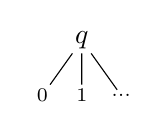
\begin{tikzpicture}[baseline=(root.base),level distance=7mm,inner ysep=0.5mm,sibling distance=5mm]
 \node (root) {$q$}
    child {node {$\scriptstyle 0$}}
    child {node {$\scriptstyle 1$}}
    child {node {$\scriptstyle \ldots$}}
;
\end{tikzpicture}$
\hspace{2cm}
$\sem{\nat \rightarrow \nat} = 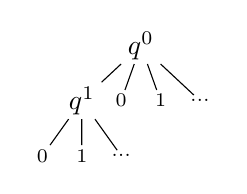
\begin{tikzpicture}[baseline=(root.base),level distance=7mm,inner ysep=0.5mm,sibling distance=5mm]
 \node (root) {$q^0$}
    child{
      node{$q^1$}
      child{node {$\scriptstyle 0$} }
      child{node {$\scriptstyle 1$} }
      child {node {$\scriptstyle \ldots$}}
    }
    child {node {$\scriptstyle 0$}}
    child {node {$\scriptstyle 1$}}
    child {node {$\scriptstyle \ldots$}}
;
\end{tikzpicture}$
\item \highlight{Play} = sequence of moves played alternatively by O and P with justification pointers.
\item \highlight{Strategy for P} = prefix-closed set of plays. $s  a  b$ in the strategy means that
P should respond $b$ when O plays $a$ in position $s$.
\item The \highlight{denotation} of a term $M$, written $\sem{M}$, is a strategy for P.
\item $\sem{ 7 : \nat} = \{ \epsilon, q, q\ 7 \}$\\
$\sem{ \pcfsucc : \nat \rightarrow \nat} = Pref( \{ q^0 q^1 n ( n+1)
\ | \ n \in \nat \} )$
\item Compositionality: $\sem{ \pcfsucc\  7} = \sem{ \pcfsucc } ; \sem{7}$
\end{itemize}
}

\frame{
\frametitle{Game semantics: composition}

\begin{itemize}
    \item Composition is done by CSP-composition + hiding:
If $\sigma : A \typear B$ and $\mu : B \typear C$ then
$$\mbox{`` }\sigma ; \mu =  (\sigma \| \mu ) \filter A,C \mbox{ ''}$$
\pause

    \item  The \highlight{fully revealed} game denotation, written $\revsem{M}$, denotes
    the set of plays obtained by not performing hiding of internal moves during composition.

\end{itemize}



}

\def\highlightat#1#2{\temporal<#1>{#2}{\underline{#2}}{\textcolor{blue}{#2}}}

\section{The theory of traversals}

\subsection{The ingredients}

\frame{ \frametitle{Computation tree}

We fix a simply-typed term $\Gamma \vdash M: T$.

\highlight{\it Computation tree} of $M$ is the AST of its $\eta$-long normal form.
\begin{itemize}
\item The \highlight{$\eta$-expansion} of $M:A\typear B$ is $\lambda x:A . Mx :A\typear B$.
\item The \highlight{$\eta$-long normal form} of $M$ is obtained
by hereditarily $\eta$-expanding every subterm of $M$ occurring at an operand position or as the body of a $\lambda$-abstraction.
\end{itemize}

Example:
$$\vdash \lambda f^{o \typear o} .
(\lambda u^{o \typear o} . u) f : (o \typear o) \typear
o \typear o$$

\begin{columns}
\column{6cm}
Its $\eta$-long normal form is
\begin{align*}
 &\vdash  \lambda f^{o \typear o} z^o . \\
&\qquad(\lambda u^{o \typear o} v^o . u (\lambda.v)) \\
&\qquad(\lambda y^o. f y) \\
&\qquad(\lambda.z) \\
&: (o \typear o) \typear o \typear o
\end{align*}

\column{4cm}
The computation tree is:
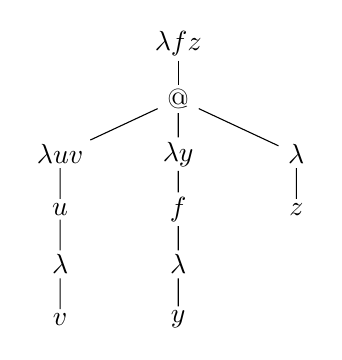
\begin{tikzpicture}[level distance=7mm,inner ysep=0.5mm]
 \node {$\lambda f z$}
    child {
        node {@}
        child {
            node {$\lambda u v$}
            child{
                node{$u$}
                child {
                    node{$\lambda$}
                    child {
                        node{$v$}
                    }
                }
            }
        }
        child {
            node {$\lambda y$}
            child{
                node {$f$}
                child{
                    node {$\lambda$}
                    child { node {$y$} }
                }
            }
        }
        child {
            node {$\lambda$}
            child{ node {$z$} }
            }
        };
\end{tikzpicture}
\end{columns}
}


\frame{
\frametitle{Justified sequence}

\begin{itemize}
\item  We define an \highlight{enabling relation} $\vdash$ on the set of nodes:
\begin{itemize}
  \item a bound variable is enabled by its binder;
  \item a free variable is enabled by the root $\theroot$;
  \item a lambda node  is enabled by its parent node;
  \item an @-node has no enabler.
\end{itemize}

\item Distinction between external nodes $N^{\theroot\vdash}$(hereditarily justified by the root) and the internal nodes $N^{@\vdash}$ (her.\ just.\ by an @-node).

\item A \highlight{justified sequence} is a sequence of nodes such that all the non @-nodes have a justification pointer respecting the relation $\vdash$.

\item  The analogy with game semantics is:
\begin{itemize}
\item $\lambda$-nodes $\equiv$ O-moves
\item @-nodes and variable-nodes $\equiv$ P-moves
\end{itemize}

\item Notions of alternation, P-view, O-view, P-visibility and O-visibility.
\end{itemize}
}




\frame{
\frametitle{Traversals rules}
The computation is described by a set $\travset(M)$ of justified sequences called \highlight{traversals} and given by induction over the rules:
%\begin{FramedTable}
%\noindent {\bf Initialization rules}
\begin{itemize}[]
\item\rulenamet{Empty} $\epsilon \in\travset(M)$
\item \rulenamet{Root} $\theroot \in \travset(M)$
%\end{itemize}
%\noindent {\bf Structural rules}
%\begin{itemize}[]
    \item \rulenamet{Lam} $t \cdot \lambda \overline{\xi} \in\travset(M) \implies t \cdot \lambda \overline{\xi} \cdot n \in\travset(M)$ where $n$
        is $\lambda \overline{\xi}$'s child and is justified by the only occurrence of
        its enabler in the P-view
    \item \rulenamet{App}  $t \cdot @ \in\travset(M) \implies$ \Pstr[0.4cm]{t \cdot (m) @  \cdot (n-m,40:0) n} $\in\travset(M)$.
%\end{itemize}
%\emph{\bf Input-variable rules}
%\begin{itemize}[]
\item \rulenamet{ExtVar} $t\cdot x\in\travset(M)$, $x\in N^{\theroot\vdash}_{\sf var}$ $\implies$
$t \cdot x \cdot n \in\travset(M)$
for any $\lambda$-node $n$ justified by some
occurrence of its parent node in the O-view of $t$. 

%\item \rulenamet{ContextValue} If $t_1
%\cdot x \cdot t_2 \in\travset(M)$ with pending node $x \in
%N_{\sf var}^{\theroot\vdash}$ then so is \Pstr[0.5cm]{t_1 \cdot
%(x){x} \cdot t_2 \cdot (xv-x,38:v){v_x} } for all $v \in
%\mathcal{D}$.
%\end{itemize}
%\emph{\bf Copy-cat rules}
%\begin{itemize}[]
\item\rulenamet{IntVar}
\Pstr[0.2cm]{t \cdot (n){n} \cdot (lx){\lambda \overline{x}}
    \ldots (x-lx,40:i){x_i} } $\in\travset(M)$, $x_i \in
    N_{\sf var}^{@\vdash} \implies$  \Pstr[0.5cm]{ t \cdot
(n){n} \cdot (lx){\lambda \overline{x}}  \ldots (x-lx,25:i){x_i}
    \cdot (letai-n,32:i){\lambda \overline{\eta_i}}} $\in\travset(M)$.
%\item\rulenamet{Value}
%  If \Pstr{t \cdot (m){m} \cdot (n){n}  \ldots
%(vn-n,50:v){v}_{n} } $\in\travset(M)$ where $n\in N$ then
%\Pstr[0.6cm]{t \cdot (m){m} \cdot (n){n} \ldots
%(vn-n,50:v){v}_{n} \cdot (vm-m,45:v){v}_m} $\in\travset(M)$.
\end{itemize}
%\caption[Traversal rules for the simply-typed
%lambda-calculus]{Traversal rules for the simply-typed
%$\lambda$-calculus.}
%\label{tab:trav_rules}
%\end{FramedTable}

}


\frame{
\frametitle{Example of traversal}


\begin{center}
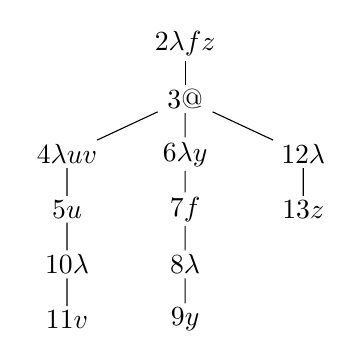
\begin{tikzpicture}[level distance=7mm,inner ysep=0.5mm]
 \node {\highlightat{2}{$\lambda f z$}}
    child {
        node {\highlightat{3}{@}}
        child {
            node {\highlightat{4}{$\lambda u v$}}
            child{
                node{\highlightat{5}{$u$}}
                child {
                    node{\highlightat{10}{$\lambda$}}
                    child {
                        node{\highlightat{11}{$v$}}
                    }
                }
            }
        }
        child {
            node {\highlightat{6}{$\lambda y$}}
            child{
                node {\highlightat{7}{$f$}}
                child{
                    node {\highlightat{8}{$\lambda$}}
                    child { node {\highlightat{9}{$y$}} }
                }
            }
        }
        child {
            node {$\highlightat{12}{\lambda}$}
            child{ node {\highlightat{13}{$z$}} }
            }
        };
\end{tikzpicture}
\end{center}

\setbox0=\hbox{$\textcolor{blue}{
\pstr{\only<2->{\nd t= (n0){\lambda f z}}
        \only<3->{\nd\cdot (n1){@}}
        \only<4->{\nd\cdot (n2-n1){\lambda u v}}
        \only<5->{\nd\cdot (n3-n2){u}}
        \only<6->{\nd\cdot (n4-n1){\lambda y}}
        \only<7->{\nd\cdot (n5-n0){f}}
        \only<8->{\nd\cdot (n6-n5){\lambda }}
        \only<9->{\nd\cdot (n7-n4){y}}
        \only<10->{\nd\cdot (n8-n3){\lambda }}
        \only<11->{\nd\cdot (n9-n2){v}}
        \only<12->{\nd\cdot (n10-n1){\lambda }}
        \only<13->{\nd\cdot (n11-n0){z}}
}}$}
\ht0 2cm\box0 % Make sure the height of box containing the traversal remains constant across the different generated slides

}

\frame{
\frametitle{Operations on traversals}
$\pstr{\nd t= (n0){\lambda f z}
        \nd\cdot (n1){@}
        \nd\cdot (n2-n1){\lambda u v}
        \nd\cdot (n3-n2){u}
        \nd\cdot (n4-n1){\lambda y}
        \nd\cdot (n5-n0){f}
        \nd\cdot (n6-n5){\lambda }
        \nd\cdot (n7-n4){y}
        \nd\cdot (n8-n3){\lambda }
        \nd\cdot (n9-n2){v}
        \nd\cdot (n10-n1){\lambda }
        \nd\cdot (n11-n0){z}
}$
\vspace*{0.4cm}
\begin{itemize}
\item The \highlight{reduction of a traversal} is obtained by keeping only
the occurrences hereditarily justified by the root:
$$ \Pstr[0.7cm]{t \filter \lambda f z = (n0){\lambda f z}\ (n1-n0){f}\ (n2-n1){\lambda }\ (n3-n0){z} }$$
\pause

\item  \highlight{\it @-nodes removal:}
$$\Pstr[0.5cm]{ t - @ = (n0){\lambda f z}\ (n1-n0){\lambda u v}\ (n2-n1){u}\ (n3-n0){\lambda y}\ (n4-n0){f}\ (n5-n4){\lambda }\ (n6-n3){y}\ (n7-n2){\lambda }\ (n8-n1){v}\ (n9-n0){\lambda }\ (n10-n0){z}}$$
\end{itemize}

}


\subsection{The Correspondence Theorem}
\frame{ \frametitle{The Correspondence Theorem}
\begin{block}{}
Let $M$ be a simply typed term of type $T$. There exists a function $\textcolor{DarkGreen}{\varphi}$
from the nodes of the \highlight{computation tree} to the
moves of the \highlight{arenas} of $\revsem{T}$ such that
$$ \textcolor{DarkGreen}{\varphi}  : \travset(M)^{-@} \textcolor{DarkGreen}{\stackrel{\cong}{\longrightarrow}}
\revsem{M} $$
$$ \textcolor{DarkGreen}{\varphi}  : \travset(M)^{\filter \theroot}  \textcolor{DarkGreen}{\stackrel{\cong}{\longrightarrow}} \sem{M} \ .$$
\end{block}
where
\begin{itemize}
\item $\highlight{\travset(M)}$ = set of traversals of the computation tree of $M$
\item $\highlight{\travset(M)^{\filter \theroot}} = \{ t \filter t_0 \ | \  t\in\travset(M) \}$
\item $\highlight{\travset(M)^{-@}} = \{ t - @ \ | \  t \in {\travset(M)} \}$
\item $\highlight{\sem{M}}$ = game-semantic denotation of $M$
\item $\highlight{
\revsem{M}}$ = revealed denotation of $M$.
\end{itemize}

}


\frame{ \frametitle{More correspondences}
\begin{center}
\begin{tabular}{c|c}
Computation tree notions & Game-semantic equivalents \\ \hline \hline \\
computation tree & revealed arena \\ \\
traversal & uncovered play \\ \\
reduced traversal & play \\ \\
path in the computation tree & P-view of an uncovered play
\end{tabular}
\end{center}
\note{Innocence $\leftrightarrow$ the next node to visit after a $\lambda$-node is determined by the current position in the syntax tree.}
}


\subsection{Example}
\frame{\frametitle{Example:
 $\vdash \lambda f^{o \typear o} .
(\lambda u^{o \typear o} . u) f : (o^4 \typear o^3) \typear
o^2 \typear o^1$}

Left: computation tree. Right: arena.
\begin{center}
\begin{tikzpicture}[level distance=7mm,inner ysep=0.5mm,inner xsep=0.5mm,sibling distance=10mm]
\node (root) {\only<2->{\color{red}}
$\lambda f z$}
    child{
      node{\only<2->{\color{red}}$@$}
          child{
            node {$\lambda u v$}
            child{
              node (u) {$u$}
              child{
                node (lmd) {$\lambda$}
                child{
                  node {$v$}
                }
              }
            }
          }
          child{
            node {$\lambda y$}
            child{
                node (h) {$f$}
                child{
                  node (h1) {$\lambda$}
                  child{
                    node {$y$}
                  }
                }
            }
          }
          child{
            node {\only<2->{\color{red}}$\lambda$}
            child{
              node (z) {\only<2->{\color{red}}$z$}
            }
          }
      }
;
\draw +(5,0) node (q1) {$q^1$}
    [level distance=20mm]
      child{
        node (q3) {$q^3$}
        [level distance=10mm]
        child{ node (q4) {$q^4$} }
      }
      child{ node (q2) {$q^2$} }
;
\only<3->{
\color{DarkGreen}
\draw[->] (root) -- node[above] {$\varphi$} (q1);
\draw[->] (h) to [bend right=20]  (q3);
\draw[->] (h1) to [bend right=20]  (q4);
\draw[->] (z) to [bend right=20]  (q2);
}
\end{tikzpicture}
\end{center}
\begin{itemize}
\item $\pstr{\nd t= (n0){\lambda f z}
        \nd\cdot (n1){@}
        \nd\cdot (n2-n1,35){\lambda u v}
        \nd\cdot (n3-n2,35){u}
        \nd\cdot (n4-n1,35){\lambda y}
        \nd\cdot (n5-n0,35){f}
        \nd\cdot (n6-n5,35){\lambda }
        \nd\cdot (n7-n4,35){y}
        \nd\cdot (n8-n3,35){\lambda }
        \nd\cdot (n9-n2,35){v}
        \nd\cdot (n10-n1,35){\lambda }
        \nd\cdot (n11-n0,35){z}
}$

\pause
\item $\Pstr{\color{red}\pview{t} = (q1){\color{red}\lambda f z} \cdot (n2){\color{red}@}
\cdot (n9-n2,35){\color{red}\lambda}
\cdot (q2-q1,35){\color{red}z}}$
\pause

\item
$
\textcolor{DarkGreen}{
\varphi (} %\textcolor{blue}
{t \filter \lambda f z}
\textcolor{DarkGreen}{)} = \textcolor{DarkGreen}{\varphi (}
\textcolor{blue}{
\Pstr[70mm]{ (q1){\lambda f z}
            \cdot (q3-q1){f}
            \cdot (q4-q3){\lambda}
            \cdot (q2-q1){z} }
}
\textcolor{DarkGreen}{)} =
{
\Pstr[70mm]{
    (q1){q}^1\
    (q5-q1){q}^3\
    (q6-q3){q}^4\
    (q2-q1){q}^2
}}
\in {\sem{M}}.
$

\end{itemize}
}

\subsection{Demo}
\frame{\frametitle{Tool demo}
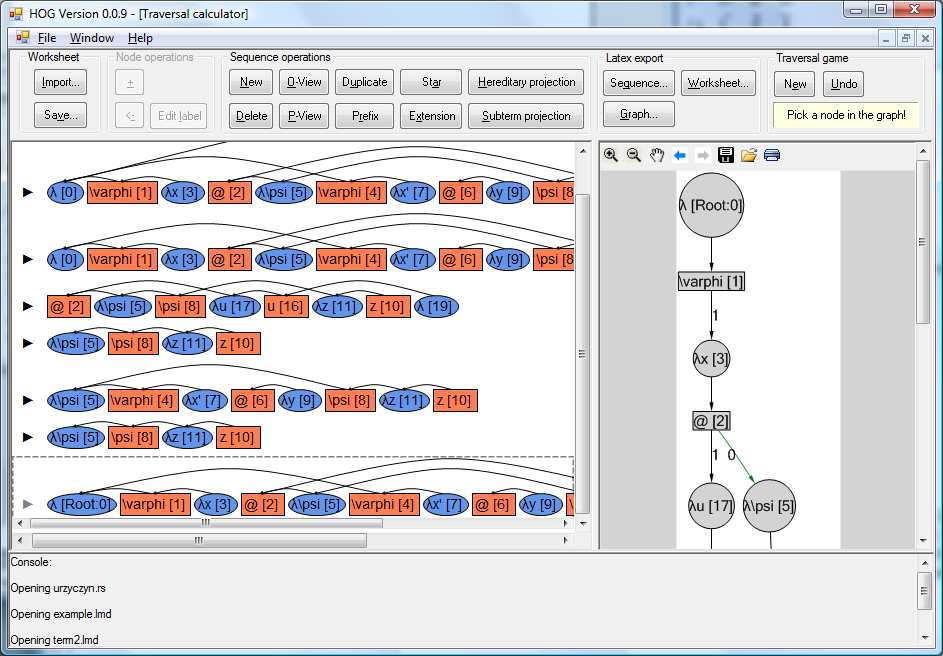
\includegraphics[width=11cm]{sshot.jpg}

}

\frame{\frametitle{Benefits}

\begin{itemize}
  \item \highlight{Pedagogical:} Game semantics is sometimes considered hard to understand. Partly because of some obscure technical definitions.
      \begin{itemize}
        \item A \highlight{P-view} is just a \highlight{control point} in the program AST. The \highlight{O-view} is the dual \ie the control point of the environment;

        \item \highlight{Innocence} means that the current control point determines the next action taken by the program.

        \item Adding reference variables breaks innocence because of side-effects.

        \item \highlight{Visibility} restricts the program to access only code that is in scope.

        \item Adding general reference breaks visibility: \eg\ $\ianew\ {\tt x} := \lambda y .y {\tt\ in\ } x~a;$

      \end{itemize}

  \item \highlight{Efficient:} top-down computation of the game denotation as opposed to a compositional bottom-up approach.
      \begin{itemize}
        \item only the relevant O-moves of the subterms are considered;
        \item hiding performed only once at the end;
        \item composition can be done at the syntactic level;
        \item traversals ending with an internal move have an O-view
        of length $\mathcal{O}(\ord{M})$.
      \end{itemize}



\end{itemize}
}

\section{Applications}
\frame{\frametitle{Applications, related works}

\begin{itemize}
\item Studying infinite structures generated by higher-order programs.
\pause

\item \highlight{Verification:}  Knapik {\it et.\ al.} (2002) showed that \highlight{MSO model checking} for trees generated by HORS
 of any order and verifying the \highlight{safety restriction} (a syntactic restriction that constrains the occurrences of variables according to their orders) is decidable.

    Using the notions of computation tree/traversal Ong was able to show (LICS06) that this result still holds in the unrestricted case.


\pause

\item Studying the effect of syntactic restrictions on the game semantics model.
 \eg\ One can show that \highlight{pointers are uniquely recoverable} in the game denotation of terms satisfying the safety restriction.
\pause

\end{itemize}

\highlight{Related works:}

\begin{itemize}
\item Stirling recently proved decidability of higher-order pattern matching with a game-semantic approach
 relying on equivalent notions of computation tree and traversal.
\end{itemize}
}



\section{Conclusion}

\frame{ \frametitle{Conclusion \& Future Works}

\begin{itemize}
\item \highlight{Conclusion:} a new \highlight{concrete} way to present game semantics
based on the theory of \highlight{traversals}.

\item \highlight{Future works:} \hfill

\begin{itemize}
\item Extend the correspondence to PCF and Idealized Algol;
\item Consider the Reachability problem in the traversal setting,
\item Complexity: characterization of space-complexity classes by analyzing the length of the traversals? (See Kazushige Terui's work.);
\end{itemize}

\end{itemize}
}

\begin{frame} \frametitle<presentation>{Bibliography}

  \begin{thebibliography}{10}
  \beamertemplatearticlebibitems
    \bibitem{abramsky:game-semantics-tutorial}
    S.~Abramsky and G.~McCusker
    \newblock Game semantics, Lecture notes.
    \newblock In {\em Proceedings of the 1997 Marktoberdorf Summer School}. 1998.

    \bibitem{localbeta2008}
    W.~Blum and C.-H.~L.~Ong
    \newblock Local computation of beta-reduction
    \newblock Technical report. University of Oxford, 2008.

    \bibitem{hague-sto07}
    M.~Hague, A.S.~Murawski, C.-H.~L. Ong and O.~Serre
    \newblock Collapsible pushdown automata and recursive schemes.
    \newblock To appear, LICS2008.

    \bibitem{OngLics2006}
    C.-H.~Luke Ong
    \newblock On model-checking trees generated by higher-order recursion schemes.
    \newblock In {\em Proceedings of LICS2006.}

    \bibitem{DBLP:conf/icalp/Stirling06}
    C.~Stirling
    \newblock A game-theoretic approach to deciding higher-order matching.
    \newblock In {\em Proceedings of ICALP2006.}

  \end{thebibliography}
\end{frame}

\end{document}

\def\toolname{HOG}

\pstrSetArrowColor{black}

\title{\texorpdfstring{A Concrete Presentation of Game Semantics}{A Concrete Presentation of Game Semantics}}

\author[W. Blum, C.-H. L. Ong]{\texorpdfstring{\\ William Blum\\ \ \\
 Joint work with C.-H. Luke Ong}{William Blum}}


\institute[Oxford University -- Edinburgh University]{School of Informatics, University of Edinburgh -- Oxford University Computing Laboratory}

\date{\small \color{red}{BCTCS, 8 April 2008}}


\begin{document}

\frame{\titlepage}

\frame{\frametitle{Overview}
\begin{itemize}
  \item
Game-semantic models are \highlight{abstract} \ie independent of the syntax of the denotated term. We give here a \highlight{concrete} \ie syntactic representation of game semantics where:
\begin{itemize}
\item The arena game is `incarnated' by some abstract syntax tree of the term,
\item Uncovered plays are given by traversals over this tree.
\end{itemize}


\item A ``Correspondence Theorem'' establishes the relationship between the game-semantic and traversal models.

\item The tool \toolname\ illustrates this correspondence.
\end{itemize}

}


\begin{frame}
  \frametitle{Outline}
  \tableofcontents
\end{frame}

\AtBeginSection[] {
   \begin{frame}
     \frametitle{Outline}
     \tableofcontents[currentpart,currentsection]
   \end{frame}
 }


%%%%%%%%%%%%%%%%%%%%%%%%%%%%%%%%%%%%%%%%%%%%%%%%%
\section{Game semantics}

\frame{\frametitle{Game semantics}
 Model of programming languages based on games (Abramsky et al.; Hyland and Ong; Nickau)
\begin{itemize}
\item 2 players: \highlight{O}pponnent (system) and \highlight{P}roponent (program)
\item The term type induces an \highlight{arena} defining the possible moves
$\sem{\nat} = 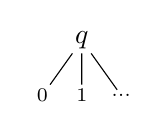
\begin{tikzpicture}[baseline=(root.base),level distance=7mm,inner ysep=0.5mm,sibling distance=5mm]
 \node (root) {$q$}
    child {node {$\scriptstyle 0$}}
    child {node {$\scriptstyle 1$}}
    child {node {$\scriptstyle \ldots$}}
;
\end{tikzpicture}$
\hspace{2cm}
$\sem{\nat \rightarrow \nat} = 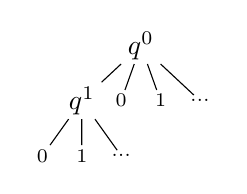
\begin{tikzpicture}[baseline=(root.base),level distance=7mm,inner ysep=0.5mm,sibling distance=5mm]
 \node (root) {$q^0$}
    child{
      node{$q^1$}
      child{node {$\scriptstyle 0$} }
      child{node {$\scriptstyle 1$} }
      child {node {$\scriptstyle \ldots$}}
    }
    child {node {$\scriptstyle 0$}}
    child {node {$\scriptstyle 1$}}
    child {node {$\scriptstyle \ldots$}}
;
\end{tikzpicture}$
\item \highlight{Play} = sequence of moves played alternatively by O and P with justification pointers.
\item \highlight{Strategy for P} = prefix-closed set of plays. $s  a  b$ in the strategy means that
P should respond $b$ when O plays $a$ in position $s$.
\item The \highlight{denotation} of a term $M$, written $\sem{M}$, is a strategy for P.
\item $\sem{ 7 : \nat} = \{ \epsilon, q, q\ 7 \}$\\
$\sem{ \pcfsucc : \nat \rightarrow \nat} = Pref( \{ q^0 q^1 n ( n+1)
\ | \ n \in \nat \} )$
\item Compositionality: $\sem{ \pcfsucc\  7} = \sem{ \pcfsucc } ; \sem{7}$
\end{itemize}
}

\frame{
\frametitle{Game semantics: composition}

\begin{itemize}
    \item Composition is done by CSP-composition + hiding:
If $\sigma : A \typear B$ and $\mu : B \typear C$ then
$$\mbox{`` }\sigma ; \mu =  (\sigma \| \mu ) \filter A,C \mbox{ ''}$$
\pause

    \item  The \highlight{fully revealed} game denotation, written $\revsem{M}$, denotes
    the set of plays obtained by not performing hiding of internal moves during composition.

\end{itemize}



}

\def\highlightat#1#2{\temporal<#1>{#2}{\underline{#2}}{\textcolor{blue}{#2}}}

\section{The theory of traversals}

\subsection{The ingredients}

\frame{ \frametitle{Computation tree}

We fix a simply-typed term $\Gamma \vdash M: T$.

\highlight{\it Computation tree} of $M$ is the AST of its $\eta$-long normal form.
\begin{itemize}
\item The \highlight{$\eta$-expansion} of $M:A\typear B$ is $\lambda x:A . Mx :A\typear B$.
\item The \highlight{$\eta$-long normal form} of $M$ is obtained
by hereditarily $\eta$-expanding every subterm of $M$ occurring at an operand position or as the body of a $\lambda$-abstraction.
\end{itemize}

Example:
$$\vdash \lambda f^{o \typear o} .
(\lambda u^{o \typear o} . u) f : (o \typear o) \typear
o \typear o$$

\begin{columns}
\column{6cm}
Its $\eta$-long normal form is
\begin{align*}
 &\vdash  \lambda f^{o \typear o} z^o . \\
&\qquad(\lambda u^{o \typear o} v^o . u (\lambda.v)) \\
&\qquad(\lambda y^o. f y) \\
&\qquad(\lambda.z) \\
&: (o \typear o) \typear o \typear o
\end{align*}

\column{4cm}
The computation tree is:
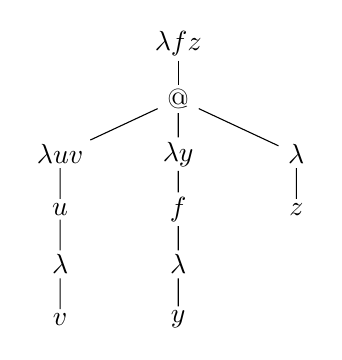
\begin{tikzpicture}[level distance=7mm,inner ysep=0.5mm]
 \node {$\lambda f z$}
    child {
        node {@}
        child {
            node {$\lambda u v$}
            child{
                node{$u$}
                child {
                    node{$\lambda$}
                    child {
                        node{$v$}
                    }
                }
            }
        }
        child {
            node {$\lambda y$}
            child{
                node {$f$}
                child{
                    node {$\lambda$}
                    child { node {$y$} }
                }
            }
        }
        child {
            node {$\lambda$}
            child{ node {$z$} }
            }
        };
\end{tikzpicture}
\end{columns}
}


\frame{
\frametitle{Justified sequence}

\begin{itemize}
\item  We define an \highlight{enabling relation} $\vdash$ on the set of nodes:
\begin{itemize}
  \item a bound variable is enabled by its binder;
  \item a free variable is enabled by the root $\theroot$;
  \item a lambda node  is enabled by its parent node;
  \item an @-node has no enabler.
\end{itemize}

\item Distinction between external nodes $N^{\theroot\vdash}$(hereditarily justified by the root) and the internal nodes $N^{@\vdash}$ (her.\ just.\ by an @-node).

\item A \highlight{justified sequence} is a sequence of nodes such that all the non @-nodes have a justification pointer respecting the relation $\vdash$.

\item  The analogy with game semantics is:
\begin{itemize}
\item $\lambda$-nodes $\equiv$ O-moves
\item @-nodes and variable-nodes $\equiv$ P-moves
\end{itemize}

\item Notions of alternation, P-view, O-view, P-visibility and O-visibility.
\end{itemize}
}




\frame{
\frametitle{Traversals rules}
The computation is described by a set $\travset(M)$ of justified sequences called \highlight{traversals} and given by induction over the rules:
%\begin{FramedTable}
%\noindent {\bf Initialization rules}
\begin{itemize}[]
\item\rulenamet{Empty} $\epsilon \in\travset(M)$
\item \rulenamet{Root} $\theroot \in \travset(M)$
%\end{itemize}
%\noindent {\bf Structural rules}
%\begin{itemize}[]
    \item \rulenamet{Lam} $t \cdot \lambda \overline{\xi} \in\travset(M) \implies t \cdot \lambda \overline{\xi} \cdot n \in\travset(M)$ where $n$
        is $\lambda \overline{\xi}$'s child and is justified by the only occurrence of
        its enabler in the P-view
    \item \rulenamet{App}  $t \cdot @ \in\travset(M) \implies$ \Pstr[0.4cm]{t \cdot (m) @  \cdot (n-m,40:0) n} $\in\travset(M)$.
%\end{itemize}
%\emph{\bf Input-variable rules}
%\begin{itemize}[]
\item \rulenamet{ExtVar} $t\cdot x\in\travset(M)$, $x\in N^{\theroot\vdash}_{\sf var}$ $\implies$
$t \cdot x \cdot n \in\travset(M)$
for any $\lambda$-node $n$ justified by some
occurrence of its parent node in the O-view of $t$. 

%\item \rulenamet{ContextValue} If $t_1
%\cdot x \cdot t_2 \in\travset(M)$ with pending node $x \in
%N_{\sf var}^{\theroot\vdash}$ then so is \Pstr[0.5cm]{t_1 \cdot
%(x){x} \cdot t_2 \cdot (xv-x,38:v){v_x} } for all $v \in
%\mathcal{D}$.
%\end{itemize}
%\emph{\bf Copy-cat rules}
%\begin{itemize}[]
\item\rulenamet{IntVar}
\Pstr[0.2cm]{t \cdot (n){n} \cdot (lx){\lambda \overline{x}}
    \ldots (x-lx,40:i){x_i} } $\in\travset(M)$, $x_i \in
    N_{\sf var}^{@\vdash} \implies$  \Pstr[0.5cm]{ t \cdot
(n){n} \cdot (lx){\lambda \overline{x}}  \ldots (x-lx,25:i){x_i}
    \cdot (letai-n,32:i){\lambda \overline{\eta_i}}} $\in\travset(M)$.
%\item\rulenamet{Value}
%  If \Pstr{t \cdot (m){m} \cdot (n){n}  \ldots
%(vn-n,50:v){v}_{n} } $\in\travset(M)$ where $n\in N$ then
%\Pstr[0.6cm]{t \cdot (m){m} \cdot (n){n} \ldots
%(vn-n,50:v){v}_{n} \cdot (vm-m,45:v){v}_m} $\in\travset(M)$.
\end{itemize}
%\caption[Traversal rules for the simply-typed
%lambda-calculus]{Traversal rules for the simply-typed
%$\lambda$-calculus.}
%\label{tab:trav_rules}
%\end{FramedTable}

}


\frame{
\frametitle{Example of traversal}


\begin{center}
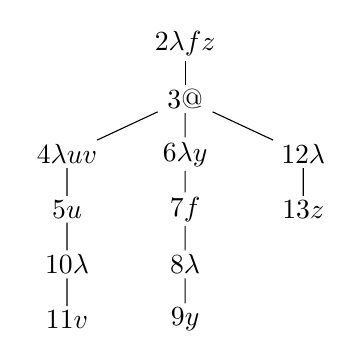
\begin{tikzpicture}[level distance=7mm,inner ysep=0.5mm]
 \node {\highlightat{2}{$\lambda f z$}}
    child {
        node {\highlightat{3}{@}}
        child {
            node {\highlightat{4}{$\lambda u v$}}
            child{
                node{\highlightat{5}{$u$}}
                child {
                    node{\highlightat{10}{$\lambda$}}
                    child {
                        node{\highlightat{11}{$v$}}
                    }
                }
            }
        }
        child {
            node {\highlightat{6}{$\lambda y$}}
            child{
                node {\highlightat{7}{$f$}}
                child{
                    node {\highlightat{8}{$\lambda$}}
                    child { node {\highlightat{9}{$y$}} }
                }
            }
        }
        child {
            node {$\highlightat{12}{\lambda}$}
            child{ node {\highlightat{13}{$z$}} }
            }
        };
\end{tikzpicture}
\end{center}

\setbox0=\hbox{$\textcolor{blue}{
\pstr{\only<2->{\nd t= (n0){\lambda f z}}
        \only<3->{\nd\cdot (n1){@}}
        \only<4->{\nd\cdot (n2-n1){\lambda u v}}
        \only<5->{\nd\cdot (n3-n2){u}}
        \only<6->{\nd\cdot (n4-n1){\lambda y}}
        \only<7->{\nd\cdot (n5-n0){f}}
        \only<8->{\nd\cdot (n6-n5){\lambda }}
        \only<9->{\nd\cdot (n7-n4){y}}
        \only<10->{\nd\cdot (n8-n3){\lambda }}
        \only<11->{\nd\cdot (n9-n2){v}}
        \only<12->{\nd\cdot (n10-n1){\lambda }}
        \only<13->{\nd\cdot (n11-n0){z}}
}}$}
\ht0 2cm\box0 % Make sure the height of box containing the traversal remains constant across the different generated slides

}

\frame{
\frametitle{Operations on traversals}
$\pstr{\nd t= (n0){\lambda f z}
        \nd\cdot (n1){@}
        \nd\cdot (n2-n1){\lambda u v}
        \nd\cdot (n3-n2){u}
        \nd\cdot (n4-n1){\lambda y}
        \nd\cdot (n5-n0){f}
        \nd\cdot (n6-n5){\lambda }
        \nd\cdot (n7-n4){y}
        \nd\cdot (n8-n3){\lambda }
        \nd\cdot (n9-n2){v}
        \nd\cdot (n10-n1){\lambda }
        \nd\cdot (n11-n0){z}
}$
\vspace*{0.4cm}
\begin{itemize}
\item The \highlight{reduction of a traversal} is obtained by keeping only
the occurrences hereditarily justified by the root:
$$ \Pstr[0.7cm]{t \filter \lambda f z = (n0){\lambda f z}\ (n1-n0){f}\ (n2-n1){\lambda }\ (n3-n0){z} }$$
\pause

\item  \highlight{\it @-nodes removal:}
$$\Pstr[0.5cm]{ t - @ = (n0){\lambda f z}\ (n1-n0){\lambda u v}\ (n2-n1){u}\ (n3-n0){\lambda y}\ (n4-n0){f}\ (n5-n4){\lambda }\ (n6-n3){y}\ (n7-n2){\lambda }\ (n8-n1){v}\ (n9-n0){\lambda }\ (n10-n0){z}}$$
\end{itemize}

}


\subsection{The Correspondence Theorem}
\frame{ \frametitle{The Correspondence Theorem}
\begin{block}{}
Let $M$ be a simply typed term of type $T$. There exists a function $\textcolor{DarkGreen}{\varphi}$
from the nodes of the \highlight{computation tree} to the
moves of the \highlight{arenas} of $\revsem{T}$ such that
$$ \textcolor{DarkGreen}{\varphi}  : \travset(M)^{-@} \textcolor{DarkGreen}{\stackrel{\cong}{\longrightarrow}}
\revsem{M} $$
$$ \textcolor{DarkGreen}{\varphi}  : \travset(M)^{\filter \theroot}  \textcolor{DarkGreen}{\stackrel{\cong}{\longrightarrow}} \sem{M} \ .$$
\end{block}
where
\begin{itemize}
\item $\highlight{\travset(M)}$ = set of traversals of the computation tree of $M$
\item $\highlight{\travset(M)^{\filter \theroot}} = \{ t \filter t_0 \ | \  t\in\travset(M) \}$
\item $\highlight{\travset(M)^{-@}} = \{ t - @ \ | \  t \in {\travset(M)} \}$
\item $\highlight{\sem{M}}$ = game-semantic denotation of $M$
\item $\highlight{
\revsem{M}}$ = revealed denotation of $M$.
\end{itemize}

}


\frame{ \frametitle{More correspondences}
\begin{center}
\begin{tabular}{c|c}
Computation tree notions & Game-semantic equivalents \\ \hline \hline \\
computation tree & revealed arena \\ \\
traversal & uncovered play \\ \\
reduced traversal & play \\ \\
path in the computation tree & P-view of an uncovered play
\end{tabular}
\end{center}
\note{Innocence $\leftrightarrow$ the next node to visit after a $\lambda$-node is determined by the current position in the syntax tree.}
}


\subsection{Example}
\frame{\frametitle{Example:
 $\vdash \lambda f^{o \typear o} .
(\lambda u^{o \typear o} . u) f : (o^4 \typear o^3) \typear
o^2 \typear o^1$}

Left: computation tree. Right: arena.
\begin{center}
\begin{tikzpicture}[level distance=7mm,inner ysep=0.5mm,inner xsep=0.5mm,sibling distance=10mm]
\node (root) {\only<2->{\color{red}}
$\lambda f z$}
    child{
      node{\only<2->{\color{red}}$@$}
          child{
            node {$\lambda u v$}
            child{
              node (u) {$u$}
              child{
                node (lmd) {$\lambda$}
                child{
                  node {$v$}
                }
              }
            }
          }
          child{
            node {$\lambda y$}
            child{
                node (h) {$f$}
                child{
                  node (h1) {$\lambda$}
                  child{
                    node {$y$}
                  }
                }
            }
          }
          child{
            node {\only<2->{\color{red}}$\lambda$}
            child{
              node (z) {\only<2->{\color{red}}$z$}
            }
          }
      }
;
\draw +(5,0) node (q1) {$q^1$}
    [level distance=20mm]
      child{
        node (q3) {$q^3$}
        [level distance=10mm]
        child{ node (q4) {$q^4$} }
      }
      child{ node (q2) {$q^2$} }
;
\only<3->{
\color{DarkGreen}
\draw[->] (root) -- node[above] {$\varphi$} (q1);
\draw[->] (h) to [bend right=20]  (q3);
\draw[->] (h1) to [bend right=20]  (q4);
\draw[->] (z) to [bend right=20]  (q2);
}
\end{tikzpicture}
\end{center}
\begin{itemize}
\item $\pstr{\nd t= (n0){\lambda f z}
        \nd\cdot (n1){@}
        \nd\cdot (n2-n1,35){\lambda u v}
        \nd\cdot (n3-n2,35){u}
        \nd\cdot (n4-n1,35){\lambda y}
        \nd\cdot (n5-n0,35){f}
        \nd\cdot (n6-n5,35){\lambda }
        \nd\cdot (n7-n4,35){y}
        \nd\cdot (n8-n3,35){\lambda }
        \nd\cdot (n9-n2,35){v}
        \nd\cdot (n10-n1,35){\lambda }
        \nd\cdot (n11-n0,35){z}
}$

\pause
\item $\Pstr{\color{red}\pview{t} = (q1){\color{red}\lambda f z} \cdot (n2){\color{red}@}
\cdot (n9-n2,35){\color{red}\lambda}
\cdot (q2-q1,35){\color{red}z}}$
\pause

\item
$
\textcolor{DarkGreen}{
\varphi (} %\textcolor{blue}
{t \filter \lambda f z}
\textcolor{DarkGreen}{)} = \textcolor{DarkGreen}{\varphi (}
\textcolor{blue}{
\Pstr[70mm]{ (q1){\lambda f z}
            \cdot (q3-q1){f}
            \cdot (q4-q3){\lambda}
            \cdot (q2-q1){z} }
}
\textcolor{DarkGreen}{)} =
{
\Pstr[70mm]{
    (q1){q}^1\
    (q5-q1){q}^3\
    (q6-q3){q}^4\
    (q2-q1){q}^2
}}
\in {\sem{M}}.
$

\end{itemize}
}

\subsection{Demo}
\frame{\frametitle{Tool demo}
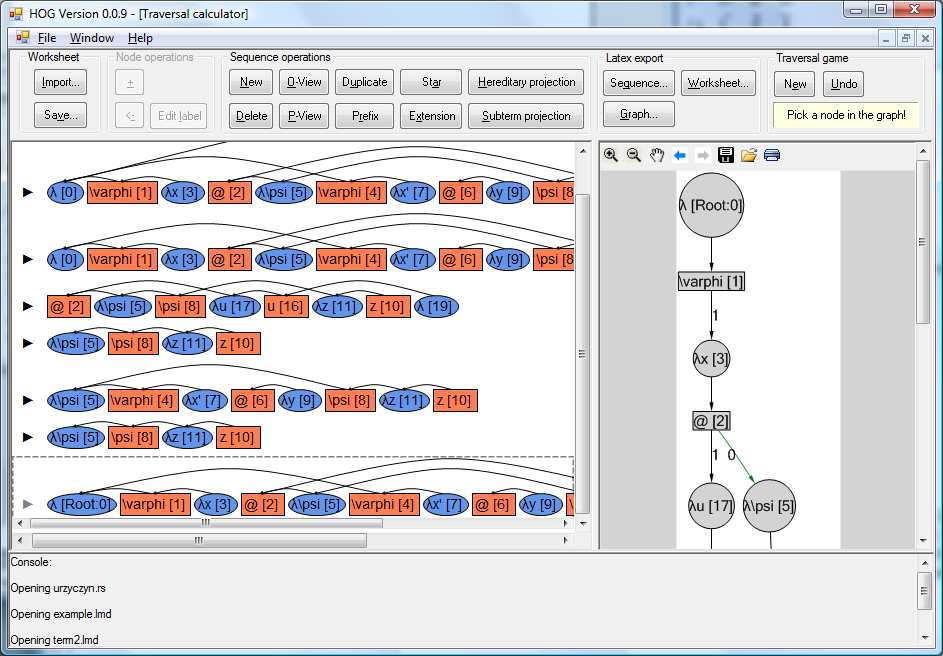
\includegraphics[width=11cm]{sshot.jpg}

}

\frame{\frametitle{Benefits}

\begin{itemize}
  \item \highlight{Pedagogical:} Game semantics is sometimes considered hard to understand. Partly because of some obscure technical definitions.
      \begin{itemize}
        \item A \highlight{P-view} is just a \highlight{control point} in the program AST. The \highlight{O-view} is the dual \ie the control point of the environment;

        \item \highlight{Innocence} means that the current control point determines the next action taken by the program.

        \item Adding reference variables breaks innocence because of side-effects.

        \item \highlight{Visibility} restricts the program to access only code that is in scope.

        \item Adding general reference breaks visibility: \eg\ $\ianew\ {\tt x} := \lambda y .y {\tt\ in\ } x~a;$

      \end{itemize}

  \item \highlight{Efficient:} top-down computation of the game denotation as opposed to a compositional bottom-up approach.
      \begin{itemize}
        \item only the relevant O-moves of the subterms are considered;
        \item hiding performed only once at the end;
        \item composition can be done at the syntactic level;
        \item traversals ending with an internal move have an O-view
        of length $\mathcal{O}(\ord{M})$.
      \end{itemize}



\end{itemize}
}

\section{Applications}
\frame{\frametitle{Applications, related works}

\begin{itemize}
\item Studying infinite structures generated by higher-order programs.
\pause

\item \highlight{Verification:}  Knapik {\it et.\ al.} (2002) showed that \highlight{MSO model checking} for trees generated by HORS
 of any order and verifying the \highlight{safety restriction} (a syntactic restriction that constrains the occurrences of variables according to their orders) is decidable.

    Using the notions of computation tree/traversal Ong was able to show (LICS06) that this result still holds in the unrestricted case.


\pause

\item Studying the effect of syntactic restrictions on the game semantics model.
 \eg\ One can show that \highlight{pointers are uniquely recoverable} in the game denotation of terms satisfying the safety restriction.
\pause

\end{itemize}

\highlight{Related works:}

\begin{itemize}
\item Stirling recently proved decidability of higher-order pattern matching with a game-semantic approach
 relying on equivalent notions of computation tree and traversal.
\end{itemize}
}



\section{Conclusion}

\frame{ \frametitle{Conclusion \& Future Works}

\begin{itemize}
\item \highlight{Conclusion:} a new \highlight{concrete} way to present game semantics
based on the theory of \highlight{traversals}.

\item \highlight{Future works:} \hfill

\begin{itemize}
\item Extend the correspondence to PCF and Idealized Algol;
\item Consider the Reachability problem in the traversal setting,
\item Complexity: characterization of space-complexity classes by analyzing the length of the traversals? (See Kazushige Terui's work.);
\end{itemize}

\end{itemize}
}

\begin{frame} \frametitle<presentation>{Bibliography}

  \begin{thebibliography}{10}
  \beamertemplatearticlebibitems
    \bibitem{abramsky:game-semantics-tutorial}
    S.~Abramsky and G.~McCusker
    \newblock Game semantics, Lecture notes.
    \newblock In {\em Proceedings of the 1997 Marktoberdorf Summer School}. 1998.

    \bibitem{localbeta2008}
    W.~Blum and C.-H.~L.~Ong
    \newblock Local computation of beta-reduction
    \newblock Technical report. University of Oxford, 2008.

    \bibitem{hague-sto07}
    M.~Hague, A.S.~Murawski, C.-H.~L. Ong and O.~Serre
    \newblock Collapsible pushdown automata and recursive schemes.
    \newblock To appear, LICS2008.

    \bibitem{OngLics2006}
    C.-H.~Luke Ong
    \newblock On model-checking trees generated by higher-order recursion schemes.
    \newblock In {\em Proceedings of LICS2006.}

    \bibitem{DBLP:conf/icalp/Stirling06}
    C.~Stirling
    \newblock A game-theoretic approach to deciding higher-order matching.
    \newblock In {\em Proceedings of ICALP2006.}

  \end{thebibliography}
\end{frame}

\end{document}

\def\toolname{HOG}

\pstrSetArrowColor{black}

\title{\texorpdfstring{A Concrete Presentation of Game Semantics}{A Concrete Presentation of Game Semantics}}

\author[W. Blum, C.-H. L. Ong]{\texorpdfstring{\\ William Blum\\ \ \\
 Joint work with C.-H. Luke Ong}{William Blum}}


\institute[Oxford University -- Edinburgh University]{School of Informatics, University of Edinburgh -- Oxford University Computing Laboratory}

\date{\small \color{red}{BCTCS, 8 April 2008}}


\begin{document}

\frame{\titlepage}

\frame{\frametitle{Overview}
\begin{itemize}
  \item
Game-semantic models are \highlight{abstract} \ie independent of the syntax of the denotated term. We give here a \highlight{concrete} \ie syntactic representation of game semantics where:
\begin{itemize}
\item The arena game is `incarnated' by some abstract syntax tree of the term,
\item Uncovered plays are given by traversals over this tree.
\end{itemize}


\item A ``Correspondence Theorem'' establishes the relationship between the game-semantic and traversal models.

\item The tool \toolname\ illustrates this correspondence.
\end{itemize}

}


\begin{frame}
  \frametitle{Outline}
  \tableofcontents
\end{frame}

\AtBeginSection[] {
   \begin{frame}
     \frametitle{Outline}
     \tableofcontents[currentpart,currentsection]
   \end{frame}
 }


%%%%%%%%%%%%%%%%%%%%%%%%%%%%%%%%%%%%%%%%%%%%%%%%%
\section{Game semantics}

\frame{\frametitle{Game semantics}
 Model of programming languages based on games (Abramsky et al.; Hyland and Ong; Nickau)
\begin{itemize}
\item 2 players: \highlight{O}pponnent (system) and \highlight{P}roponent (program)
\item The term type induces an \highlight{arena} defining the possible moves
$\sem{\nat} = 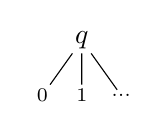
\begin{tikzpicture}[baseline=(root.base),level distance=7mm,inner ysep=0.5mm,sibling distance=5mm]
 \node (root) {$q$}
    child {node {$\scriptstyle 0$}}
    child {node {$\scriptstyle 1$}}
    child {node {$\scriptstyle \ldots$}}
;
\end{tikzpicture}$
\hspace{2cm}
$\sem{\nat \rightarrow \nat} = 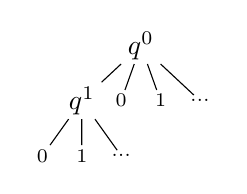
\begin{tikzpicture}[baseline=(root.base),level distance=7mm,inner ysep=0.5mm,sibling distance=5mm]
 \node (root) {$q^0$}
    child{
      node{$q^1$}
      child{node {$\scriptstyle 0$} }
      child{node {$\scriptstyle 1$} }
      child {node {$\scriptstyle \ldots$}}
    }
    child {node {$\scriptstyle 0$}}
    child {node {$\scriptstyle 1$}}
    child {node {$\scriptstyle \ldots$}}
;
\end{tikzpicture}$
\item \highlight{Play} = sequence of moves played alternatively by O and P with justification pointers.
\item \highlight{Strategy for P} = prefix-closed set of plays. $s  a  b$ in the strategy means that
P should respond $b$ when O plays $a$ in position $s$.
\item The \highlight{denotation} of a term $M$, written $\sem{M}$, is a strategy for P.
\item $\sem{ 7 : \nat} = \{ \epsilon, q, q\ 7 \}$\\
$\sem{ \pcfsucc : \nat \rightarrow \nat} = Pref( \{ q^0 q^1 n ( n+1)
\ | \ n \in \nat \} )$
\item Compositionality: $\sem{ \pcfsucc\  7} = \sem{ \pcfsucc } ; \sem{7}$
\end{itemize}
}

\frame{
\frametitle{Game semantics: composition}

\begin{itemize}
    \item Composition is done by CSP-composition + hiding:
If $\sigma : A \typear B$ and $\mu : B \typear C$ then
$$\mbox{`` }\sigma ; \mu =  (\sigma \| \mu ) \filter A,C \mbox{ ''}$$
\pause

    \item  The \highlight{fully revealed} game denotation, written $\revsem{M}$, denotes
    the set of plays obtained by not performing hiding of internal moves during composition.

\end{itemize}



}

\def\highlightat#1#2{\temporal<#1>{#2}{\underline{#2}}{\textcolor{blue}{#2}}}

\section{The theory of traversals}

\subsection{The ingredients}

\frame{ \frametitle{Computation tree}

We fix a simply-typed term $\Gamma \vdash M: T$.

\highlight{\it Computation tree} of $M$ is the AST of its $\eta$-long normal form.
\begin{itemize}
\item The \highlight{$\eta$-expansion} of $M:A\typear B$ is $\lambda x:A . Mx :A\typear B$.
\item The \highlight{$\eta$-long normal form} of $M$ is obtained
by hereditarily $\eta$-expanding every subterm of $M$ occurring at an operand position or as the body of a $\lambda$-abstraction.
\end{itemize}

Example:
$$\vdash \lambda f^{o \typear o} .
(\lambda u^{o \typear o} . u) f : (o \typear o) \typear
o \typear o$$

\begin{columns}
\column{6cm}
Its $\eta$-long normal form is
\begin{align*}
 &\vdash  \lambda f^{o \typear o} z^o . \\
&\qquad(\lambda u^{o \typear o} v^o . u (\lambda.v)) \\
&\qquad(\lambda y^o. f y) \\
&\qquad(\lambda.z) \\
&: (o \typear o) \typear o \typear o
\end{align*}

\column{4cm}
The computation tree is:
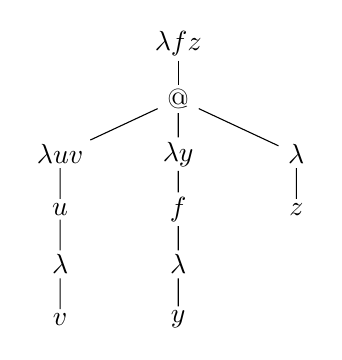
\begin{tikzpicture}[level distance=7mm,inner ysep=0.5mm]
 \node {$\lambda f z$}
    child {
        node {@}
        child {
            node {$\lambda u v$}
            child{
                node{$u$}
                child {
                    node{$\lambda$}
                    child {
                        node{$v$}
                    }
                }
            }
        }
        child {
            node {$\lambda y$}
            child{
                node {$f$}
                child{
                    node {$\lambda$}
                    child { node {$y$} }
                }
            }
        }
        child {
            node {$\lambda$}
            child{ node {$z$} }
            }
        };
\end{tikzpicture}
\end{columns}
}


\frame{
\frametitle{Justified sequence}

\begin{itemize}
\item  We define an \highlight{enabling relation} $\vdash$ on the set of nodes:
\begin{itemize}
  \item a bound variable is enabled by its binder;
  \item a free variable is enabled by the root $\theroot$;
  \item a lambda node  is enabled by its parent node;
  \item an @-node has no enabler.
\end{itemize}

\item Distinction between external nodes $N^{\theroot\vdash}$(hereditarily justified by the root) and the internal nodes $N^{@\vdash}$ (her.\ just.\ by an @-node).

\item A \highlight{justified sequence} is a sequence of nodes such that all the non @-nodes have a justification pointer respecting the relation $\vdash$.

\item  The analogy with game semantics is:
\begin{itemize}
\item $\lambda$-nodes $\equiv$ O-moves
\item @-nodes and variable-nodes $\equiv$ P-moves
\end{itemize}

\item Notions of alternation, P-view, O-view, P-visibility and O-visibility.
\end{itemize}
}




\frame{
\frametitle{Traversals rules}
The computation is described by a set $\travset(M)$ of justified sequences called \highlight{traversals} and given by induction over the rules:
%\begin{FramedTable}
%\noindent {\bf Initialization rules}
\begin{itemize}[]
\item\rulenamet{Empty} $\epsilon \in\travset(M)$
\item \rulenamet{Root} $\theroot \in \travset(M)$
%\end{itemize}
%\noindent {\bf Structural rules}
%\begin{itemize}[]
    \item \rulenamet{Lam} $t \cdot \lambda \overline{\xi} \in\travset(M) \implies t \cdot \lambda \overline{\xi} \cdot n \in\travset(M)$ where $n$
        is $\lambda \overline{\xi}$'s child and is justified by the only occurrence of
        its enabler in the P-view
    \item \rulenamet{App}  $t \cdot @ \in\travset(M) \implies$ \Pstr[0.4cm]{t \cdot (m) @  \cdot (n-m,40:0) n} $\in\travset(M)$.
%\end{itemize}
%\emph{\bf Input-variable rules}
%\begin{itemize}[]
\item \rulenamet{ExtVar} $t\cdot x\in\travset(M)$, $x\in N^{\theroot\vdash}_{\sf var}$ $\implies$
$t \cdot x \cdot n \in\travset(M)$
for any $\lambda$-node $n$ justified by some
occurrence of its parent node in the O-view of $t$. 

%\item \rulenamet{ContextValue} If $t_1
%\cdot x \cdot t_2 \in\travset(M)$ with pending node $x \in
%N_{\sf var}^{\theroot\vdash}$ then so is \Pstr[0.5cm]{t_1 \cdot
%(x){x} \cdot t_2 \cdot (xv-x,38:v){v_x} } for all $v \in
%\mathcal{D}$.
%\end{itemize}
%\emph{\bf Copy-cat rules}
%\begin{itemize}[]
\item\rulenamet{IntVar}
\Pstr[0.2cm]{t \cdot (n){n} \cdot (lx){\lambda \overline{x}}
    \ldots (x-lx,40:i){x_i} } $\in\travset(M)$, $x_i \in
    N_{\sf var}^{@\vdash} \implies$  \Pstr[0.5cm]{ t \cdot
(n){n} \cdot (lx){\lambda \overline{x}}  \ldots (x-lx,25:i){x_i}
    \cdot (letai-n,32:i){\lambda \overline{\eta_i}}} $\in\travset(M)$.
%\item\rulenamet{Value}
%  If \Pstr{t \cdot (m){m} \cdot (n){n}  \ldots
%(vn-n,50:v){v}_{n} } $\in\travset(M)$ where $n\in N$ then
%\Pstr[0.6cm]{t \cdot (m){m} \cdot (n){n} \ldots
%(vn-n,50:v){v}_{n} \cdot (vm-m,45:v){v}_m} $\in\travset(M)$.
\end{itemize}
%\caption[Traversal rules for the simply-typed
%lambda-calculus]{Traversal rules for the simply-typed
%$\lambda$-calculus.}
%\label{tab:trav_rules}
%\end{FramedTable}

}


\frame{
\frametitle{Example of traversal}


\begin{center}
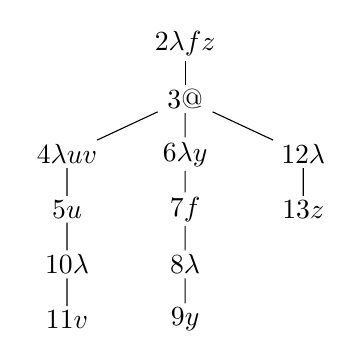
\begin{tikzpicture}[level distance=7mm,inner ysep=0.5mm]
 \node {\highlightat{2}{$\lambda f z$}}
    child {
        node {\highlightat{3}{@}}
        child {
            node {\highlightat{4}{$\lambda u v$}}
            child{
                node{\highlightat{5}{$u$}}
                child {
                    node{\highlightat{10}{$\lambda$}}
                    child {
                        node{\highlightat{11}{$v$}}
                    }
                }
            }
        }
        child {
            node {\highlightat{6}{$\lambda y$}}
            child{
                node {\highlightat{7}{$f$}}
                child{
                    node {\highlightat{8}{$\lambda$}}
                    child { node {\highlightat{9}{$y$}} }
                }
            }
        }
        child {
            node {$\highlightat{12}{\lambda}$}
            child{ node {\highlightat{13}{$z$}} }
            }
        };
\end{tikzpicture}
\end{center}

\setbox0=\hbox{$\textcolor{blue}{
\pstr{\only<2->{\nd t= (n0){\lambda f z}}
        \only<3->{\nd\cdot (n1){@}}
        \only<4->{\nd\cdot (n2-n1){\lambda u v}}
        \only<5->{\nd\cdot (n3-n2){u}}
        \only<6->{\nd\cdot (n4-n1){\lambda y}}
        \only<7->{\nd\cdot (n5-n0){f}}
        \only<8->{\nd\cdot (n6-n5){\lambda }}
        \only<9->{\nd\cdot (n7-n4){y}}
        \only<10->{\nd\cdot (n8-n3){\lambda }}
        \only<11->{\nd\cdot (n9-n2){v}}
        \only<12->{\nd\cdot (n10-n1){\lambda }}
        \only<13->{\nd\cdot (n11-n0){z}}
}}$}
\ht0 2cm\box0 % Make sure the height of box containing the traversal remains constant across the different generated slides

}

\frame{
\frametitle{Operations on traversals}
$\pstr{\nd t= (n0){\lambda f z}
        \nd\cdot (n1){@}
        \nd\cdot (n2-n1){\lambda u v}
        \nd\cdot (n3-n2){u}
        \nd\cdot (n4-n1){\lambda y}
        \nd\cdot (n5-n0){f}
        \nd\cdot (n6-n5){\lambda }
        \nd\cdot (n7-n4){y}
        \nd\cdot (n8-n3){\lambda }
        \nd\cdot (n9-n2){v}
        \nd\cdot (n10-n1){\lambda }
        \nd\cdot (n11-n0){z}
}$
\vspace*{0.4cm}
\begin{itemize}
\item The \highlight{reduction of a traversal} is obtained by keeping only
the occurrences hereditarily justified by the root:
$$ \Pstr[0.7cm]{t \filter \lambda f z = (n0){\lambda f z}\ (n1-n0){f}\ (n2-n1){\lambda }\ (n3-n0){z} }$$
\pause

\item  \highlight{\it @-nodes removal:}
$$\Pstr[0.5cm]{ t - @ = (n0){\lambda f z}\ (n1-n0){\lambda u v}\ (n2-n1){u}\ (n3-n0){\lambda y}\ (n4-n0){f}\ (n5-n4){\lambda }\ (n6-n3){y}\ (n7-n2){\lambda }\ (n8-n1){v}\ (n9-n0){\lambda }\ (n10-n0){z}}$$
\end{itemize}

}


\subsection{The Correspondence Theorem}
\frame{ \frametitle{The Correspondence Theorem}
\begin{block}{}
Let $M$ be a simply typed term of type $T$. There exists a function $\textcolor{DarkGreen}{\varphi}$
from the nodes of the \highlight{computation tree} to the
moves of the \highlight{arenas} of $\revsem{T}$ such that
$$ \textcolor{DarkGreen}{\varphi}  : \travset(M)^{-@} \textcolor{DarkGreen}{\stackrel{\cong}{\longrightarrow}}
\revsem{M} $$
$$ \textcolor{DarkGreen}{\varphi}  : \travset(M)^{\filter \theroot}  \textcolor{DarkGreen}{\stackrel{\cong}{\longrightarrow}} \sem{M} \ .$$
\end{block}
where
\begin{itemize}
\item $\highlight{\travset(M)}$ = set of traversals of the computation tree of $M$
\item $\highlight{\travset(M)^{\filter \theroot}} = \{ t \filter t_0 \ | \  t\in\travset(M) \}$
\item $\highlight{\travset(M)^{-@}} = \{ t - @ \ | \  t \in {\travset(M)} \}$
\item $\highlight{\sem{M}}$ = game-semantic denotation of $M$
\item $\highlight{
\revsem{M}}$ = revealed denotation of $M$.
\end{itemize}

}


\frame{ \frametitle{More correspondences}
\begin{center}
\begin{tabular}{c|c}
Computation tree notions & Game-semantic equivalents \\ \hline \hline \\
computation tree & revealed arena \\ \\
traversal & uncovered play \\ \\
reduced traversal & play \\ \\
path in the computation tree & P-view of an uncovered play
\end{tabular}
\end{center}
\note{Innocence $\leftrightarrow$ the next node to visit after a $\lambda$-node is determined by the current position in the syntax tree.}
}


\subsection{Example}
\frame{\frametitle{Example:
 $\vdash \lambda f^{o \typear o} .
(\lambda u^{o \typear o} . u) f : (o^4 \typear o^3) \typear
o^2 \typear o^1$}

Left: computation tree. Right: arena.
\begin{center}
\begin{tikzpicture}[level distance=7mm,inner ysep=0.5mm,inner xsep=0.5mm,sibling distance=10mm]
\node (root) {\only<2->{\color{red}}
$\lambda f z$}
    child{
      node{\only<2->{\color{red}}$@$}
          child{
            node {$\lambda u v$}
            child{
              node (u) {$u$}
              child{
                node (lmd) {$\lambda$}
                child{
                  node {$v$}
                }
              }
            }
          }
          child{
            node {$\lambda y$}
            child{
                node (h) {$f$}
                child{
                  node (h1) {$\lambda$}
                  child{
                    node {$y$}
                  }
                }
            }
          }
          child{
            node {\only<2->{\color{red}}$\lambda$}
            child{
              node (z) {\only<2->{\color{red}}$z$}
            }
          }
      }
;
\draw +(5,0) node (q1) {$q^1$}
    [level distance=20mm]
      child{
        node (q3) {$q^3$}
        [level distance=10mm]
        child{ node (q4) {$q^4$} }
      }
      child{ node (q2) {$q^2$} }
;
\only<3->{
\color{DarkGreen}
\draw[->] (root) -- node[above] {$\varphi$} (q1);
\draw[->] (h) to [bend right=20]  (q3);
\draw[->] (h1) to [bend right=20]  (q4);
\draw[->] (z) to [bend right=20]  (q2);
}
\end{tikzpicture}
\end{center}
\begin{itemize}
\item $\pstr{\nd t= (n0){\lambda f z}
        \nd\cdot (n1){@}
        \nd\cdot (n2-n1,35){\lambda u v}
        \nd\cdot (n3-n2,35){u}
        \nd\cdot (n4-n1,35){\lambda y}
        \nd\cdot (n5-n0,35){f}
        \nd\cdot (n6-n5,35){\lambda }
        \nd\cdot (n7-n4,35){y}
        \nd\cdot (n8-n3,35){\lambda }
        \nd\cdot (n9-n2,35){v}
        \nd\cdot (n10-n1,35){\lambda }
        \nd\cdot (n11-n0,35){z}
}$

\pause
\item $\Pstr{\color{red}\pview{t} = (q1){\color{red}\lambda f z} \cdot (n2){\color{red}@}
\cdot (n9-n2,35){\color{red}\lambda}
\cdot (q2-q1,35){\color{red}z}}$
\pause

\item
$
\textcolor{DarkGreen}{
\varphi (} %\textcolor{blue}
{t \filter \lambda f z}
\textcolor{DarkGreen}{)} = \textcolor{DarkGreen}{\varphi (}
\textcolor{blue}{
\Pstr[70mm]{ (q1){\lambda f z}
            \cdot (q3-q1){f}
            \cdot (q4-q3){\lambda}
            \cdot (q2-q1){z} }
}
\textcolor{DarkGreen}{)} =
{
\Pstr[70mm]{
    (q1){q}^1\
    (q5-q1){q}^3\
    (q6-q3){q}^4\
    (q2-q1){q}^2
}}
\in {\sem{M}}.
$

\end{itemize}
}

\subsection{Demo}
\frame{\frametitle{Tool demo}
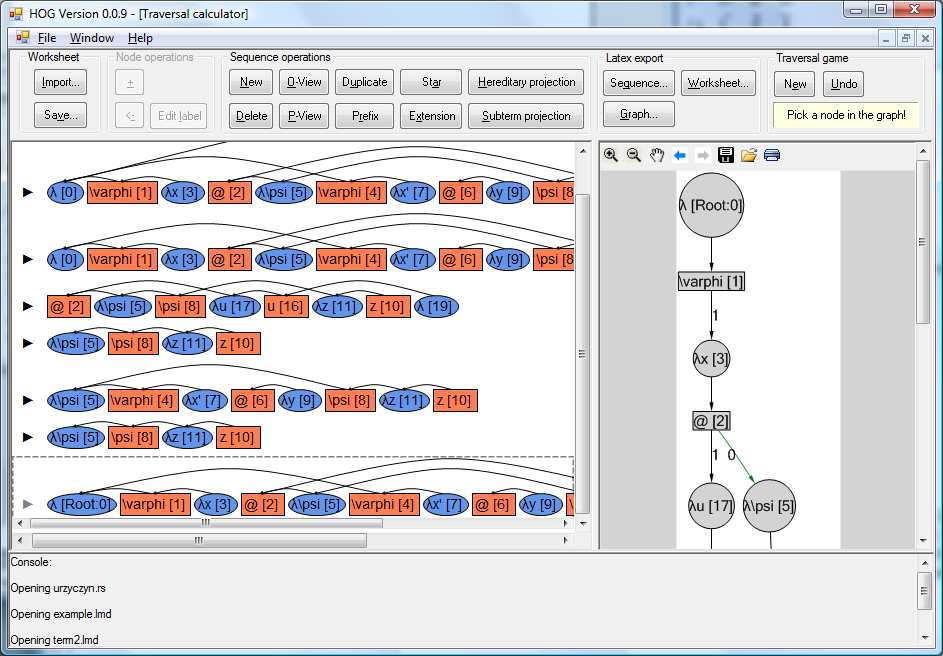
\includegraphics[width=11cm]{sshot.jpg}

}

\frame{\frametitle{Benefits}

\begin{itemize}
  \item \highlight{Pedagogical:} Game semantics is sometimes considered hard to understand. Partly because of some obscure technical definitions.
      \begin{itemize}
        \item A \highlight{P-view} is just a \highlight{control point} in the program AST. The \highlight{O-view} is the dual \ie the control point of the environment;

        \item \highlight{Innocence} means that the current control point determines the next action taken by the program.

        \item Adding reference variables breaks innocence because of side-effects.

        \item \highlight{Visibility} restricts the program to access only code that is in scope.

        \item Adding general reference breaks visibility: \eg\ $\ianew\ {\tt x} := \lambda y .y {\tt\ in\ } x~a;$

      \end{itemize}

  \item \highlight{Efficient:} top-down computation of the game denotation as opposed to a compositional bottom-up approach.
      \begin{itemize}
        \item only the relevant O-moves of the subterms are considered;
        \item hiding performed only once at the end;
        \item composition can be done at the syntactic level;
        \item traversals ending with an internal move have an O-view
        of length $\mathcal{O}(\ord{M})$.
      \end{itemize}



\end{itemize}
}

\section{Applications}
\frame{\frametitle{Applications, related works}

\begin{itemize}
\item Studying infinite structures generated by higher-order programs.
\pause

\item \highlight{Verification:}  Knapik {\it et.\ al.} (2002) showed that \highlight{MSO model checking} for trees generated by HORS
 of any order and verifying the \highlight{safety restriction} (a syntactic restriction that constrains the occurrences of variables according to their orders) is decidable.

    Using the notions of computation tree/traversal Ong was able to show (LICS06) that this result still holds in the unrestricted case.


\pause

\item Studying the effect of syntactic restrictions on the game semantics model.
 \eg\ One can show that \highlight{pointers are uniquely recoverable} in the game denotation of terms satisfying the safety restriction.
\pause

\end{itemize}

\highlight{Related works:}

\begin{itemize}
\item Stirling recently proved decidability of higher-order pattern matching with a game-semantic approach
 relying on equivalent notions of computation tree and traversal.
\end{itemize}
}



\section{Conclusion}

\frame{ \frametitle{Conclusion \& Future Works}

\begin{itemize}
\item \highlight{Conclusion:} a new \highlight{concrete} way to present game semantics
based on the theory of \highlight{traversals}.

\item \highlight{Future works:} \hfill

\begin{itemize}
\item Extend the correspondence to PCF and Idealized Algol;
\item Consider the Reachability problem in the traversal setting,
\item Complexity: characterization of space-complexity classes by analyzing the length of the traversals? (See Kazushige Terui's work.);
\end{itemize}

\end{itemize}
}

\begin{frame} \frametitle<presentation>{Bibliography}

  \begin{thebibliography}{10}
  \beamertemplatearticlebibitems
    \bibitem{abramsky:game-semantics-tutorial}
    S.~Abramsky and G.~McCusker
    \newblock Game semantics, Lecture notes.
    \newblock In {\em Proceedings of the 1997 Marktoberdorf Summer School}. 1998.

    \bibitem{localbeta2008}
    W.~Blum and C.-H.~L.~Ong
    \newblock Local computation of beta-reduction
    \newblock Technical report. University of Oxford, 2008.

    \bibitem{hague-sto07}
    M.~Hague, A.S.~Murawski, C.-H.~L. Ong and O.~Serre
    \newblock Collapsible pushdown automata and recursive schemes.
    \newblock To appear, LICS2008.

    \bibitem{OngLics2006}
    C.-H.~Luke Ong
    \newblock On model-checking trees generated by higher-order recursion schemes.
    \newblock In {\em Proceedings of LICS2006.}

    \bibitem{DBLP:conf/icalp/Stirling06}
    C.~Stirling
    \newblock A game-theoretic approach to deciding higher-order matching.
    \newblock In {\em Proceedings of ICALP2006.}

  \end{thebibliography}
\end{frame}

\end{document}

\def\toolname{HOG}

\pstrSetArrowColor{black}

\title{\texorpdfstring{A Concrete Presentation of Game Semantics}{A Concrete Presentation of Game Semantics}}

\author[W. Blum, C.-H. L. Ong]{\texorpdfstring{\\ William Blum\\ \ \\
 Joint work with C.-H. Luke Ong}{William Blum}}


\institute[Oxford University -- Edinburgh University]{School of Informatics, University of Edinburgh -- Oxford University Computing Laboratory}

\date{\small \color{red}{BCTCS, 8 April 2008}}


\begin{document}

\frame{\titlepage}

\frame{\frametitle{Overview}
\begin{itemize}
  \item
Game-semantic models are \highlight{abstract} \ie independent of the syntax of the denotated term. We give here a \highlight{concrete} \ie syntactic representation of game semantics where:
\begin{itemize}
\item The arena game is `incarnated' by some abstract syntax tree of the term,
\item Uncovered plays are given by traversals over this tree.
\end{itemize}


\item A ``Correspondence Theorem'' establishes the relationship between the game-semantic and traversal models.

\item The tool \toolname\ illustrates this correspondence.
\end{itemize}

}


\begin{frame}
  \frametitle{Outline}
  \tableofcontents
\end{frame}

\AtBeginSection[] {
   \begin{frame}
     \frametitle{Outline}
     \tableofcontents[currentpart,currentsection]
   \end{frame}
 }


%%%%%%%%%%%%%%%%%%%%%%%%%%%%%%%%%%%%%%%%%%%%%%%%%
\section{Game semantics}

\frame{\frametitle{Game semantics}
 Model of programming languages based on games (Abramsky et al.; Hyland and Ong; Nickau)
\begin{itemize}
\item 2 players: \highlight{O}pponnent (system) and \highlight{P}roponent (program)
\item The term type induces an \highlight{arena} defining the possible moves
$\sem{\nat} = 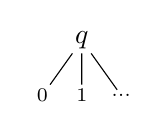
\begin{tikzpicture}[baseline=(root.base),level distance=7mm,inner ysep=0.5mm,sibling distance=5mm]
 \node (root) {$q$}
    child {node {$\scriptstyle 0$}}
    child {node {$\scriptstyle 1$}}
    child {node {$\scriptstyle \ldots$}}
;
\end{tikzpicture}$
\hspace{2cm}
$\sem{\nat \rightarrow \nat} = 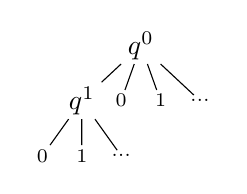
\begin{tikzpicture}[baseline=(root.base),level distance=7mm,inner ysep=0.5mm,sibling distance=5mm]
 \node (root) {$q^0$}
    child{
      node{$q^1$}
      child{node {$\scriptstyle 0$} }
      child{node {$\scriptstyle 1$} }
      child {node {$\scriptstyle \ldots$}}
    }
    child {node {$\scriptstyle 0$}}
    child {node {$\scriptstyle 1$}}
    child {node {$\scriptstyle \ldots$}}
;
\end{tikzpicture}$
\item \highlight{Play} = sequence of moves played alternatively by O and P with justification pointers.
\item \highlight{Strategy for P} = prefix-closed set of plays. $s  a  b$ in the strategy means that
P should respond $b$ when O plays $a$ in position $s$.
\item The \highlight{denotation} of a term $M$, written $\sem{M}$, is a strategy for P.
\item $\sem{ 7 : \nat} = \{ \epsilon, q, q\ 7 \}$\\
$\sem{ \pcfsucc : \nat \rightarrow \nat} = Pref( \{ q^0 q^1 n ( n+1)
\ | \ n \in \nat \} )$
\item Compositionality: $\sem{ \pcfsucc\  7} = \sem{ \pcfsucc } ; \sem{7}$
\end{itemize}
}

\frame{
\frametitle{Game semantics: composition}

\begin{itemize}
    \item Composition is done by CSP-composition + hiding:
If $\sigma : A \typear B$ and $\mu : B \typear C$ then
$$\mbox{`` }\sigma ; \mu =  (\sigma \| \mu ) \filter A,C \mbox{ ''}$$
\pause

    \item  The \highlight{fully revealed} game denotation, written $\revsem{M}$, denotes
    the set of plays obtained by not performing hiding of internal moves during composition.

\end{itemize}



}

\def\highlightat#1#2{\temporal<#1>{#2}{\underline{#2}}{\textcolor{blue}{#2}}}

\section{The theory of traversals}

\subsection{The ingredients}

\frame{ \frametitle{Computation tree}

We fix a simply-typed term $\Gamma \vdash M: T$.

\highlight{\it Computation tree} of $M$ is the AST of its $\eta$-long normal form.
\begin{itemize}
\item The \highlight{$\eta$-expansion} of $M:A\typear B$ is $\lambda x:A . Mx :A\typear B$.
\item The \highlight{$\eta$-long normal form} of $M$ is obtained
by hereditarily $\eta$-expanding every subterm of $M$ occurring at an operand position or as the body of a $\lambda$-abstraction.
\end{itemize}

Example:
$$\vdash \lambda f^{o \typear o} .
(\lambda u^{o \typear o} . u) f : (o \typear o) \typear
o \typear o$$

\begin{columns}
\column{6cm}
Its $\eta$-long normal form is
\begin{align*}
 &\vdash  \lambda f^{o \typear o} z^o . \\
&\qquad(\lambda u^{o \typear o} v^o . u (\lambda.v)) \\
&\qquad(\lambda y^o. f y) \\
&\qquad(\lambda.z) \\
&: (o \typear o) \typear o \typear o
\end{align*}

\column{4cm}
The computation tree is:
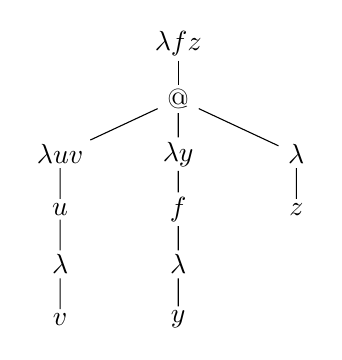
\begin{tikzpicture}[level distance=7mm,inner ysep=0.5mm]
 \node {$\lambda f z$}
    child {
        node {@}
        child {
            node {$\lambda u v$}
            child{
                node{$u$}
                child {
                    node{$\lambda$}
                    child {
                        node{$v$}
                    }
                }
            }
        }
        child {
            node {$\lambda y$}
            child{
                node {$f$}
                child{
                    node {$\lambda$}
                    child { node {$y$} }
                }
            }
        }
        child {
            node {$\lambda$}
            child{ node {$z$} }
            }
        };
\end{tikzpicture}
\end{columns}
}


\frame{
\frametitle{Justified sequence}

\begin{itemize}
\item  We define an \highlight{enabling relation} $\vdash$ on the set of nodes:
\begin{itemize}
  \item a bound variable is enabled by its binder;
  \item a free variable is enabled by the root $\theroot$;
  \item a lambda node  is enabled by its parent node;
  \item an @-node has no enabler.
\end{itemize}

\item Distinction between external nodes $N^{\theroot\vdash}$(hereditarily justified by the root) and the internal nodes $N^{@\vdash}$ (her.\ just.\ by an @-node).

\item A \highlight{justified sequence} is a sequence of nodes such that all the non @-nodes have a justification pointer respecting the relation $\vdash$.

\item  The analogy with game semantics is:
\begin{itemize}
\item $\lambda$-nodes $\equiv$ O-moves
\item @-nodes and variable-nodes $\equiv$ P-moves
\end{itemize}

\item Notions of alternation, P-view, O-view, P-visibility and O-visibility.
\end{itemize}
}




\frame{
\frametitle{Traversals rules}
The computation is described by a set $\travset(M)$ of justified sequences called \highlight{traversals} and given by induction over the rules:
%\begin{FramedTable}
%\noindent {\bf Initialization rules}
\begin{itemize}[]
\item\rulenamet{Empty} $\epsilon \in\travset(M)$
\item \rulenamet{Root} $\theroot \in \travset(M)$
%\end{itemize}
%\noindent {\bf Structural rules}
%\begin{itemize}[]
    \item \rulenamet{Lam} $t \cdot \lambda \overline{\xi} \in\travset(M) \implies t \cdot \lambda \overline{\xi} \cdot n \in\travset(M)$ where $n$
        is $\lambda \overline{\xi}$'s child and is justified by the only occurrence of
        its enabler in the P-view
    \item \rulenamet{App}  $t \cdot @ \in\travset(M) \implies$ \Pstr[0.4cm]{t \cdot (m) @  \cdot (n-m,40:0) n} $\in\travset(M)$.
%\end{itemize}
%\emph{\bf Input-variable rules}
%\begin{itemize}[]
\item \rulenamet{ExtVar} $t\cdot x\in\travset(M)$, $x\in N^{\theroot\vdash}_{\sf var}$ $\implies$
$t \cdot x \cdot n \in\travset(M)$
for any $\lambda$-node $n$ justified by some
occurrence of its parent node in the O-view of $t$. 

%\item \rulenamet{ContextValue} If $t_1
%\cdot x \cdot t_2 \in\travset(M)$ with pending node $x \in
%N_{\sf var}^{\theroot\vdash}$ then so is \Pstr[0.5cm]{t_1 \cdot
%(x){x} \cdot t_2 \cdot (xv-x,38:v){v_x} } for all $v \in
%\mathcal{D}$.
%\end{itemize}
%\emph{\bf Copy-cat rules}
%\begin{itemize}[]
\item\rulenamet{IntVar}
\Pstr[0.2cm]{t \cdot (n){n} \cdot (lx){\lambda \overline{x}}
    \ldots (x-lx,40:i){x_i} } $\in\travset(M)$, $x_i \in
    N_{\sf var}^{@\vdash} \implies$  \Pstr[0.5cm]{ t \cdot
(n){n} \cdot (lx){\lambda \overline{x}}  \ldots (x-lx,25:i){x_i}
    \cdot (letai-n,32:i){\lambda \overline{\eta_i}}} $\in\travset(M)$.
%\item\rulenamet{Value}
%  If \Pstr{t \cdot (m){m} \cdot (n){n}  \ldots
%(vn-n,50:v){v}_{n} } $\in\travset(M)$ where $n\in N$ then
%\Pstr[0.6cm]{t \cdot (m){m} \cdot (n){n} \ldots
%(vn-n,50:v){v}_{n} \cdot (vm-m,45:v){v}_m} $\in\travset(M)$.
\end{itemize}
%\caption[Traversal rules for the simply-typed
%lambda-calculus]{Traversal rules for the simply-typed
%$\lambda$-calculus.}
%\label{tab:trav_rules}
%\end{FramedTable}

}


\frame{
\frametitle{Example of traversal}


\begin{center}
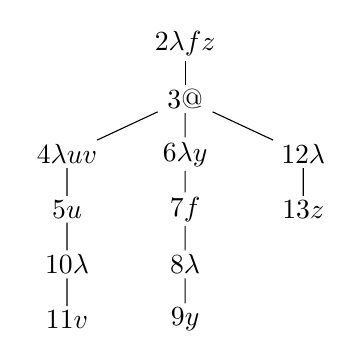
\begin{tikzpicture}[level distance=7mm,inner ysep=0.5mm]
 \node {\highlightat{2}{$\lambda f z$}}
    child {
        node {\highlightat{3}{@}}
        child {
            node {\highlightat{4}{$\lambda u v$}}
            child{
                node{\highlightat{5}{$u$}}
                child {
                    node{\highlightat{10}{$\lambda$}}
                    child {
                        node{\highlightat{11}{$v$}}
                    }
                }
            }
        }
        child {
            node {\highlightat{6}{$\lambda y$}}
            child{
                node {\highlightat{7}{$f$}}
                child{
                    node {\highlightat{8}{$\lambda$}}
                    child { node {\highlightat{9}{$y$}} }
                }
            }
        }
        child {
            node {$\highlightat{12}{\lambda}$}
            child{ node {\highlightat{13}{$z$}} }
            }
        };
\end{tikzpicture}
\end{center}

\setbox0=\hbox{$\textcolor{blue}{
\pstr{\only<2->{\nd t= (n0){\lambda f z}}
        \only<3->{\nd\cdot (n1){@}}
        \only<4->{\nd\cdot (n2-n1){\lambda u v}}
        \only<5->{\nd\cdot (n3-n2){u}}
        \only<6->{\nd\cdot (n4-n1){\lambda y}}
        \only<7->{\nd\cdot (n5-n0){f}}
        \only<8->{\nd\cdot (n6-n5){\lambda }}
        \only<9->{\nd\cdot (n7-n4){y}}
        \only<10->{\nd\cdot (n8-n3){\lambda }}
        \only<11->{\nd\cdot (n9-n2){v}}
        \only<12->{\nd\cdot (n10-n1){\lambda }}
        \only<13->{\nd\cdot (n11-n0){z}}
}}$}
\ht0 2cm\box0 % Make sure the height of box containing the traversal remains constant across the different generated slides

}

\frame{
\frametitle{Operations on traversals}
$\pstr{\nd t= (n0){\lambda f z}
        \nd\cdot (n1){@}
        \nd\cdot (n2-n1){\lambda u v}
        \nd\cdot (n3-n2){u}
        \nd\cdot (n4-n1){\lambda y}
        \nd\cdot (n5-n0){f}
        \nd\cdot (n6-n5){\lambda }
        \nd\cdot (n7-n4){y}
        \nd\cdot (n8-n3){\lambda }
        \nd\cdot (n9-n2){v}
        \nd\cdot (n10-n1){\lambda }
        \nd\cdot (n11-n0){z}
}$
\vspace*{0.4cm}
\begin{itemize}
\item The \highlight{reduction of a traversal} is obtained by keeping only
the occurrences hereditarily justified by the root:
$$ \Pstr[0.7cm]{t \filter \lambda f z = (n0){\lambda f z}\ (n1-n0){f}\ (n2-n1){\lambda }\ (n3-n0){z} }$$
\pause

\item  \highlight{\it @-nodes removal:}
$$\Pstr[0.5cm]{ t - @ = (n0){\lambda f z}\ (n1-n0){\lambda u v}\ (n2-n1){u}\ (n3-n0){\lambda y}\ (n4-n0){f}\ (n5-n4){\lambda }\ (n6-n3){y}\ (n7-n2){\lambda }\ (n8-n1){v}\ (n9-n0){\lambda }\ (n10-n0){z}}$$
\end{itemize}

}


\subsection{The Correspondence Theorem}
\frame{ \frametitle{The Correspondence Theorem}
\begin{block}{}
Let $M$ be a simply typed term of type $T$. There exists a function $\textcolor{DarkGreen}{\varphi}$
from the nodes of the \highlight{computation tree} to the
moves of the \highlight{arenas} of $\revsem{T}$ such that
$$ \textcolor{DarkGreen}{\varphi}  : \travset(M)^{-@} \textcolor{DarkGreen}{\stackrel{\cong}{\longrightarrow}}
\revsem{M} $$
$$ \textcolor{DarkGreen}{\varphi}  : \travset(M)^{\filter \theroot}  \textcolor{DarkGreen}{\stackrel{\cong}{\longrightarrow}} \sem{M} \ .$$
\end{block}
where
\begin{itemize}
\item $\highlight{\travset(M)}$ = set of traversals of the computation tree of $M$
\item $\highlight{\travset(M)^{\filter \theroot}} = \{ t \filter t_0 \ | \  t\in\travset(M) \}$
\item $\highlight{\travset(M)^{-@}} = \{ t - @ \ | \  t \in {\travset(M)} \}$
\item $\highlight{\sem{M}}$ = game-semantic denotation of $M$
\item $\highlight{
\revsem{M}}$ = revealed denotation of $M$.
\end{itemize}

}


\frame{ \frametitle{More correspondences}
\begin{center}
\begin{tabular}{c|c}
Computation tree notions & Game-semantic equivalents \\ \hline \hline \\
computation tree & revealed arena \\ \\
traversal & uncovered play \\ \\
reduced traversal & play \\ \\
path in the computation tree & P-view of an uncovered play
\end{tabular}
\end{center}
\note{Innocence $\leftrightarrow$ the next node to visit after a $\lambda$-node is determined by the current position in the syntax tree.}
}


\subsection{Example}
\frame{\frametitle{Example:
 $\vdash \lambda f^{o \typear o} .
(\lambda u^{o \typear o} . u) f : (o^4 \typear o^3) \typear
o^2 \typear o^1$}

Left: computation tree. Right: arena.
\begin{center}
\begin{tikzpicture}[level distance=7mm,inner ysep=0.5mm,inner xsep=0.5mm,sibling distance=10mm]
\node (root) {\only<2->{\color{red}}
$\lambda f z$}
    child{
      node{\only<2->{\color{red}}$@$}
          child{
            node {$\lambda u v$}
            child{
              node (u) {$u$}
              child{
                node (lmd) {$\lambda$}
                child{
                  node {$v$}
                }
              }
            }
          }
          child{
            node {$\lambda y$}
            child{
                node (h) {$f$}
                child{
                  node (h1) {$\lambda$}
                  child{
                    node {$y$}
                  }
                }
            }
          }
          child{
            node {\only<2->{\color{red}}$\lambda$}
            child{
              node (z) {\only<2->{\color{red}}$z$}
            }
          }
      }
;
\draw +(5,0) node (q1) {$q^1$}
    [level distance=20mm]
      child{
        node (q3) {$q^3$}
        [level distance=10mm]
        child{ node (q4) {$q^4$} }
      }
      child{ node (q2) {$q^2$} }
;
\only<3->{
\color{DarkGreen}
\draw[->] (root) -- node[above] {$\varphi$} (q1);
\draw[->] (h) to [bend right=20]  (q3);
\draw[->] (h1) to [bend right=20]  (q4);
\draw[->] (z) to [bend right=20]  (q2);
}
\end{tikzpicture}
\end{center}
\begin{itemize}
\item $\pstr{\nd t= (n0){\lambda f z}
        \nd\cdot (n1){@}
        \nd\cdot (n2-n1,35){\lambda u v}
        \nd\cdot (n3-n2,35){u}
        \nd\cdot (n4-n1,35){\lambda y}
        \nd\cdot (n5-n0,35){f}
        \nd\cdot (n6-n5,35){\lambda }
        \nd\cdot (n7-n4,35){y}
        \nd\cdot (n8-n3,35){\lambda }
        \nd\cdot (n9-n2,35){v}
        \nd\cdot (n10-n1,35){\lambda }
        \nd\cdot (n11-n0,35){z}
}$

\pause
\item $\Pstr{\color{red}\pview{t} = (q1){\color{red}\lambda f z} \cdot (n2){\color{red}@}
\cdot (n9-n2,35){\color{red}\lambda}
\cdot (q2-q1,35){\color{red}z}}$
\pause

\item
$
\textcolor{DarkGreen}{
\varphi (} %\textcolor{blue}
{t \filter \lambda f z}
\textcolor{DarkGreen}{)} = \textcolor{DarkGreen}{\varphi (}
\textcolor{blue}{
\Pstr[70mm]{ (q1){\lambda f z}
            \cdot (q3-q1){f}
            \cdot (q4-q3){\lambda}
            \cdot (q2-q1){z} }
}
\textcolor{DarkGreen}{)} =
{
\Pstr[70mm]{
    (q1){q}^1\
    (q5-q1){q}^3\
    (q6-q3){q}^4\
    (q2-q1){q}^2
}}
\in {\sem{M}}.
$

\end{itemize}
}

\subsection{Demo}
\frame{\frametitle{Tool demo}
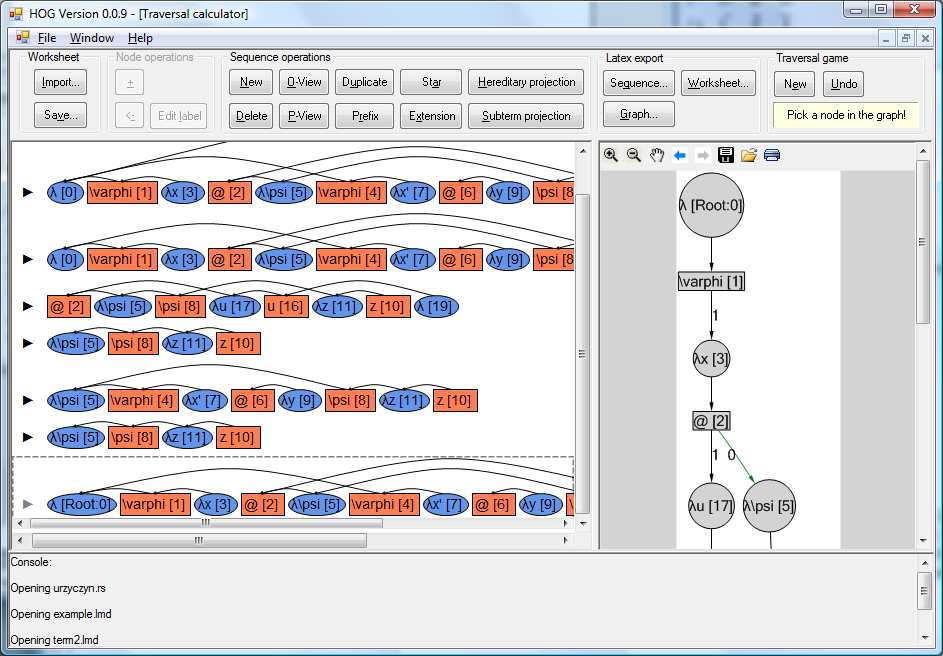
\includegraphics[width=11cm]{sshot.jpg}

}

\frame{\frametitle{Benefits}

\begin{itemize}
  \item \highlight{Pedagogical:} Game semantics is sometimes considered hard to understand. Partly because of some obscure technical definitions.
      \begin{itemize}
        \item A \highlight{P-view} is just a \highlight{control point} in the program AST. The \highlight{O-view} is the dual \ie the control point of the environment;

        \item \highlight{Innocence} means that the current control point determines the next action taken by the program.

        \item Adding reference variables breaks innocence because of side-effects.

        \item \highlight{Visibility} restricts the program to access only code that is in scope.

        \item Adding general reference breaks visibility: \eg\ $\ianew\ {\tt x} := \lambda y .y {\tt\ in\ } x~a;$

      \end{itemize}

  \item \highlight{Efficient:} top-down computation of the game denotation as opposed to a compositional bottom-up approach.
      \begin{itemize}
        \item only the relevant O-moves of the subterms are considered;
        \item hiding performed only once at the end;
        \item composition can be done at the syntactic level;
        \item traversals ending with an internal move have an O-view
        of length $\mathcal{O}(\ord{M})$.
      \end{itemize}



\end{itemize}
}

\section{Applications}
\frame{\frametitle{Applications, related works}

\begin{itemize}
\item Studying infinite structures generated by higher-order programs.
\pause

\item \highlight{Verification:}  Knapik {\it et.\ al.} (2002) showed that \highlight{MSO model checking} for trees generated by HORS
 of any order and verifying the \highlight{safety restriction} (a syntactic restriction that constrains the occurrences of variables according to their orders) is decidable.

    Using the notions of computation tree/traversal Ong was able to show (LICS06) that this result still holds in the unrestricted case.


\pause

\item Studying the effect of syntactic restrictions on the game semantics model.
 \eg\ One can show that \highlight{pointers are uniquely recoverable} in the game denotation of terms satisfying the safety restriction.
\pause

\end{itemize}

\highlight{Related works:}

\begin{itemize}
\item Stirling recently proved decidability of higher-order pattern matching with a game-semantic approach
 relying on equivalent notions of computation tree and traversal.
\end{itemize}
}



\section{Conclusion}

\frame{ \frametitle{Conclusion \& Future Works}

\begin{itemize}
\item \highlight{Conclusion:} a new \highlight{concrete} way to present game semantics
based on the theory of \highlight{traversals}.

\item \highlight{Future works:} \hfill

\begin{itemize}
\item Extend the correspondence to PCF and Idealized Algol;
\item Consider the Reachability problem in the traversal setting,
\item Complexity: characterization of space-complexity classes by analyzing the length of the traversals? (See Kazushige Terui's work.);
\end{itemize}

\end{itemize}
}

\begin{frame} \frametitle<presentation>{Bibliography}

  \begin{thebibliography}{10}
  \beamertemplatearticlebibitems
    \bibitem{abramsky:game-semantics-tutorial}
    S.~Abramsky and G.~McCusker
    \newblock Game semantics, Lecture notes.
    \newblock In {\em Proceedings of the 1997 Marktoberdorf Summer School}. 1998.

    \bibitem{localbeta2008}
    W.~Blum and C.-H.~L.~Ong
    \newblock Local computation of beta-reduction
    \newblock Technical report. University of Oxford, 2008.

    \bibitem{hague-sto07}
    M.~Hague, A.S.~Murawski, C.-H.~L. Ong and O.~Serre
    \newblock Collapsible pushdown automata and recursive schemes.
    \newblock To appear, LICS2008.

    \bibitem{OngLics2006}
    C.-H.~Luke Ong
    \newblock On model-checking trees generated by higher-order recursion schemes.
    \newblock In {\em Proceedings of LICS2006.}

    \bibitem{DBLP:conf/icalp/Stirling06}
    C.~Stirling
    \newblock A game-theoretic approach to deciding higher-order matching.
    \newblock In {\em Proceedings of ICALP2006.}

  \end{thebibliography}
\end{frame}

\end{document}
